% \documentclass[journal]{vgtc}                % final (journal style)
% \documentclass[review,journal]{vgtc}         % review (journal style)
% \documentclass[widereview]{vgtc}             % wide-spaced review
% \documentclass[preprint,journal]{vgtc}       % preprint (journal style)
% First we choose the document class (can be book, report, article etc.)
\documentclass[11pt]{article}
% \documentclass[11pt, twocolumn]{elsarticle}
% \documentclass{ieeetran}

\usepackage{mathtools} % Math
\usepackage{amssymb} % More Math symbols
\usepackage{textgreek} % Greek letters inline with text
\usepackage{graphics} % Images
\usepackage{pythonhighlight} % Syntax Highlighted code
\usepackage[margin=1in]{geometry} % Change Margins

% \ifpdf%                                % if we use pdflatex
%   \pdfoutput=1\relax                   % create PDFs from pdfLaTeX
%   \pdfcompresslevel=9                  % PDF Compression
%   \pdfoptionpdfminorversion=7          % create PDF 1.7
%   \ExecuteOptions{pdftex}
%   \usepackage{graphicx}                % allow us to embed graphics files
%   \DeclareGraphicsExtensions{.pdf,.png,.jpg,.jpeg} % for pdflatex we expect .pdf, .png, or .jpg files
% \else%                                 % else we use pure latex
%   \ExecuteOptions{dvips}
%   \usepackage{graphicx}                % allow us to embed graphics files
%   \DeclareGraphicsExtensions{.eps}     % for pure latex we expect eps files
% \fi%

%% it is recomended to use ``\autoref{sec:bla}'' instead of ``Fig.~\ref{sec:bla}''
% \graphicspath{{figures/}{pictures/}{images/}{./}} % where to search for the images
\usepackage{microtype}                 % use micro-typography (slightly more compact, better to read)
\PassOptionsToPackage{warn}{textcomp}  % to address font issues with \textrightarrow
\usepackage{textcomp}                  % use better special symbols
\usepackage{mathptmx}                  % use matching math font
\usepackage{times}                     % we use Times as the main font
\renewcommand*\ttdefault{txtt}         % a nicer typewriter font
\usepackage{cite}                      % needed to automatically sort the references


\title{Title of my document}
% \date{2019-0}
\author{Flavio R. de A. F. Mello}


%% Paper title.
% \title{Global Illumination for Fun and Profit}

%% This is how authors are specified in the journal style

%% indicate IEEE Member or Student Member in form indicated below
% \author{Roy G. Biv, Ed Grimley, \textit{Member, IEEE}, and Martha Stewart}
% \authorfooter{
% %% insert punctuation at end of each item
% \item
%  Roy G. Biv is with Starbucks Research. E-mail: roy.g.biv@aol.com.
% \item
%  Ed Grimley is with Grimley Widgets, Inc.. E-mail: ed.grimley@aol.com.
% \item
%  Martha Stewart is with Martha Stewart Enterprises at Microsoft
%  Research. E-mail: martha.stewart@marthastewart.com.
% }

%other entries to be set up for journal
% \shortauthortitle{Biv \MakeLowercase{\textit{et al.}}: Global Illumination for Fun and Profit}

% \abstract{Duis au}

% Now we start the main document stuff
\begin{document}

\maketitle

\section{Domain and Task}
    This work aims to study the implementation of a Reinforcement Learning algorithm in a multi-agent scenario. For this study, a simple task was devised: agents are randomly placed in the playing field and their goal is to reach a particular desired arrangement. The environment is discrete, static, and fully observable by all agents. States are deterministic and episodic in nature.

\subsection{Playing Field Arrangement}
    The field consists of 7 locations arranged in a cross-shaped form.

    \begin{figure}[h]
        \centering
        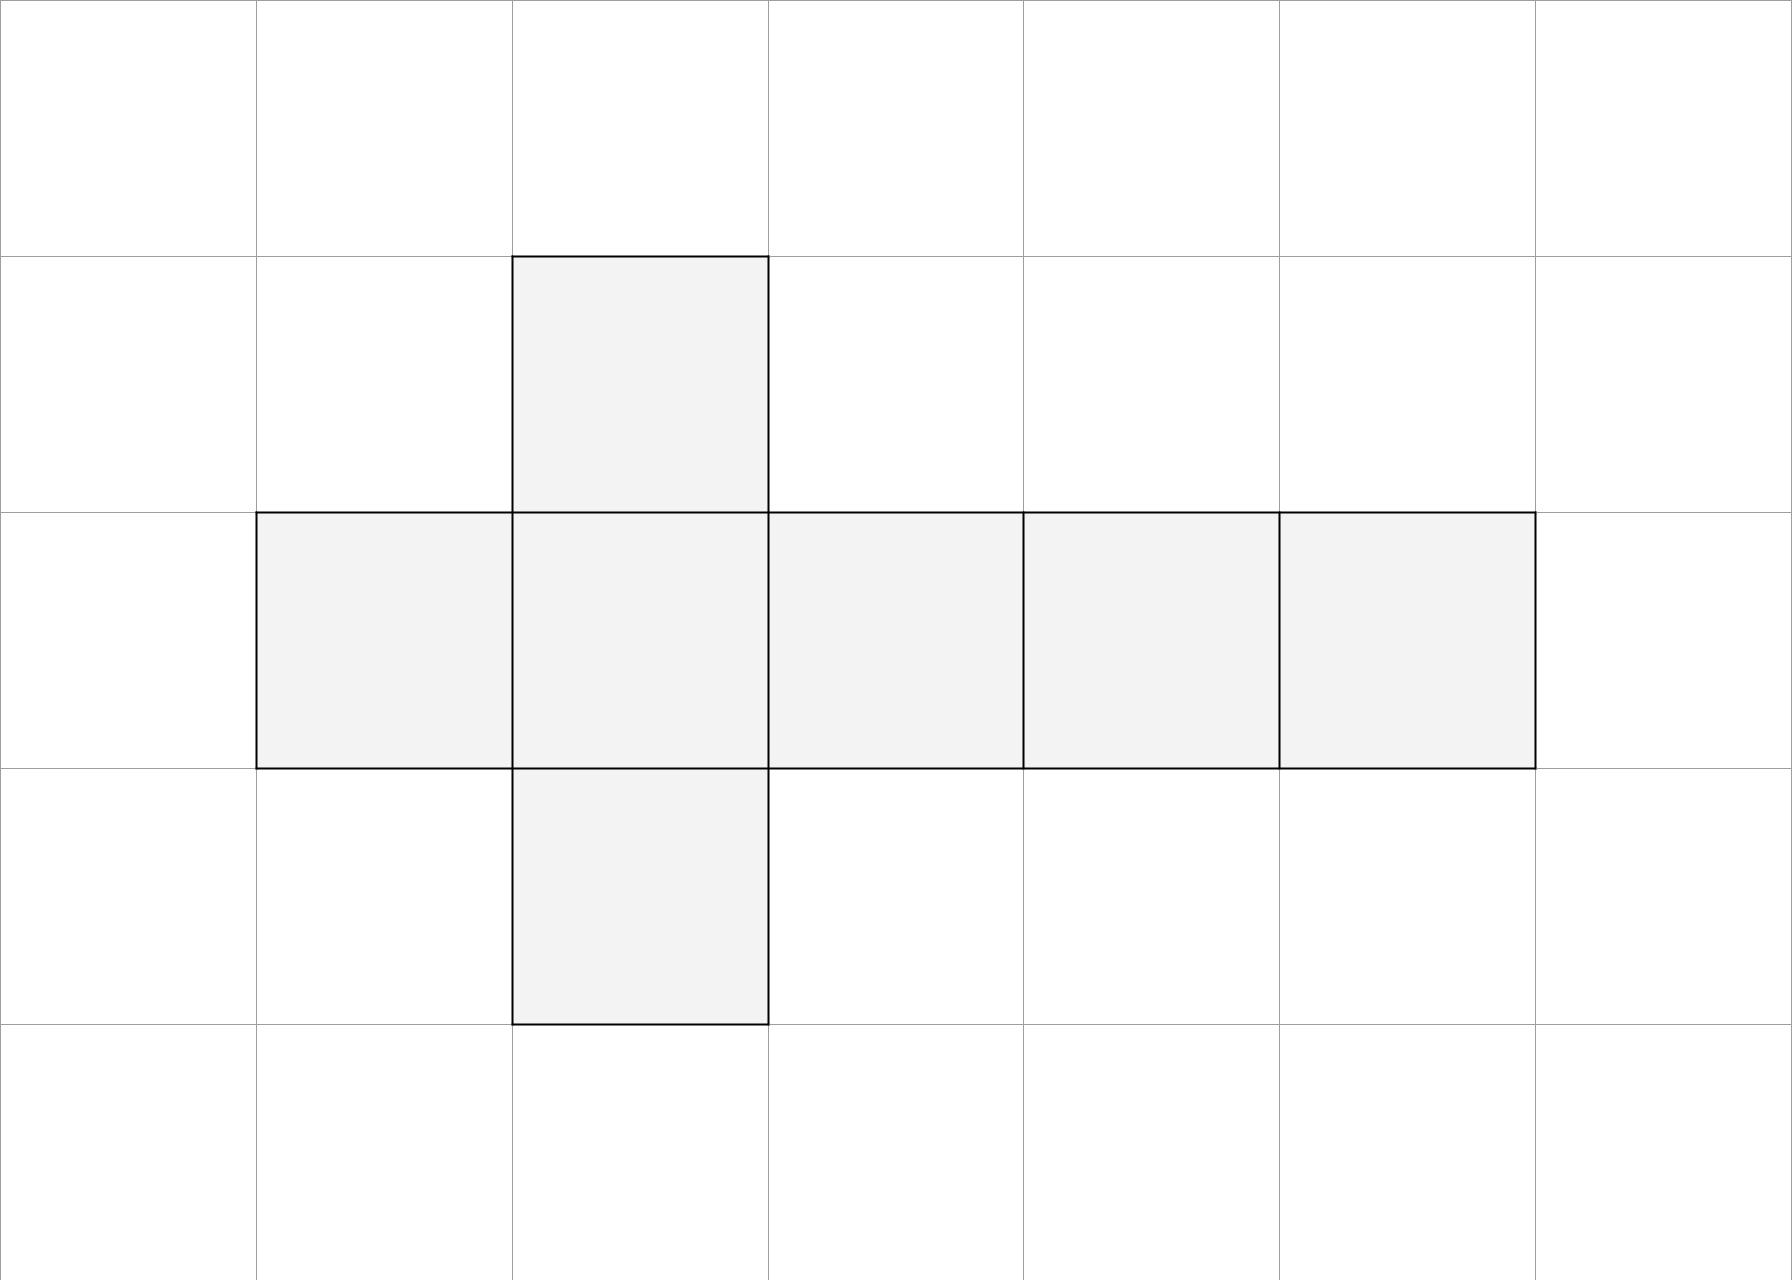
\includegraphics[height=4cm]{./Images/1_Playing_Field.jpg}
        \caption{Visual representation of the playing field}
    \end{figure}

\subsection{Playing Rules}
    Each action consists of a move to an adjacent location. Moves are only allowed in the cardinal directions, no diagonal moves are allowed. Multiple agents may not occupy a same location at the same time, therefore moves are only allowed if the destination is an empty location. Alternatively, agents may elect to stay in the same place. Thus, there are 5 possible actions: move up, move right, move down, move left, and stay in the same place. It is important to note that the field topology plays a role in determining which actions are possible for a given agent in a given state. It is perfectly possible for agents' action options be reduced to staying in place for a specific state. Agents will take turns performing actions, starting with agent 1.

\subsection{Task Goal}
    The goal is to have the agents reach the rightmost section of the field in ordered section. The agent with the smallest id number is to be at the rightmost square, followed by the other agents successively. The rightmost section is a narrow corridor, this setup allows for situations where a given agent may block the passage of the other. This characteristic of the playing field was intentionally designed to require for cooperation between agents. If they directly move to their final position, one agent may be blocking the another agent's path and thus fail to reach the final desired state.

% // IMAGE task goal for 1, 2 & 3 agents


\section{State Transition and Reward Functions} \label{sec:transition}
    For implementation purposes, the states are encoded into a single string of 7 characters. Agents are assigned ids in the form of positive numbers, which are used to indicate their position in the field. the value `0` is reserved for empty spaces. Each of the 7 locations is assigned an id from 0 through 6, which is used to map the location with the index in the encoded string. Figures \ref{fig:field_indexed} and \ref{fig:field_mapping} show the location indexes and an example of the mapping between a state string and its equivalent board arrangement.


    \begin{figure}[h]
        \centering
        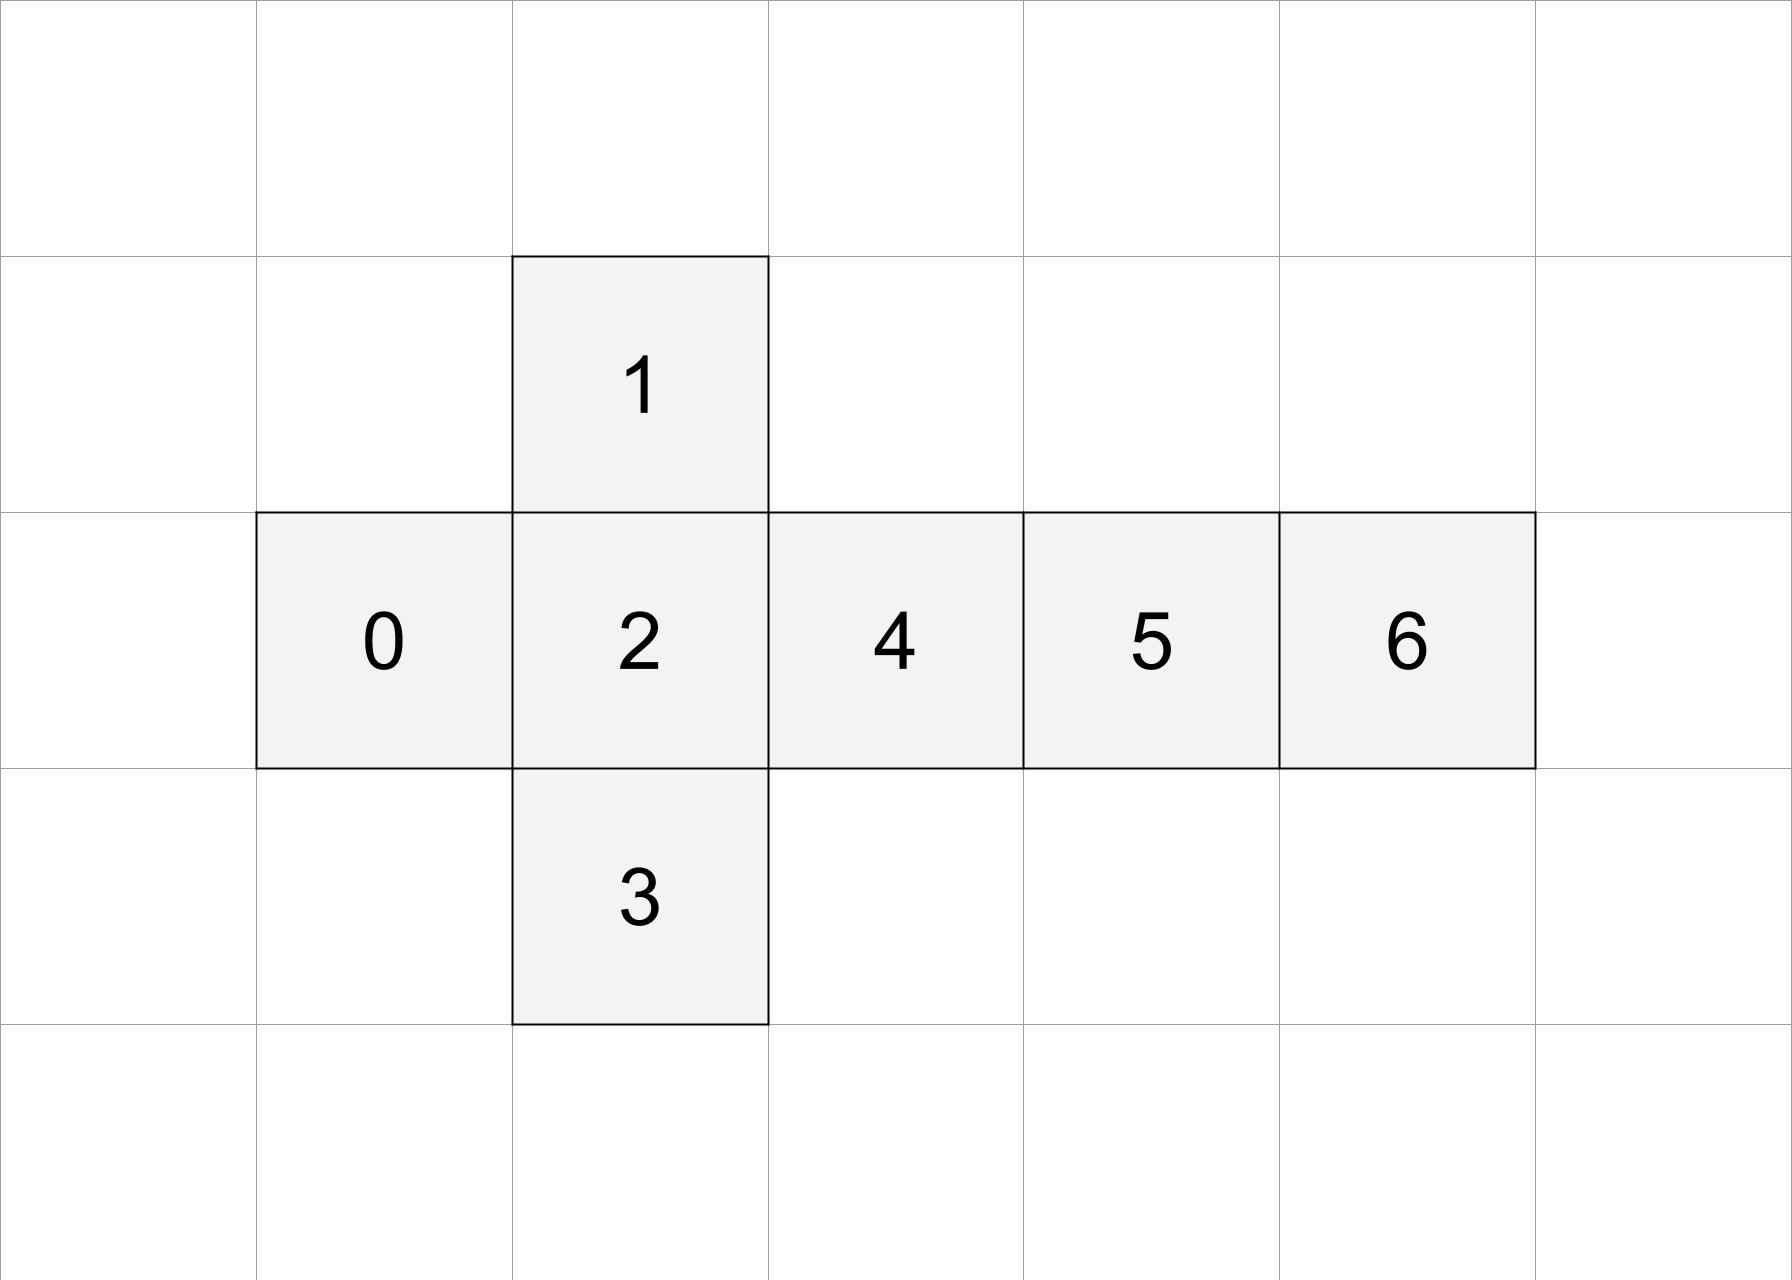
\includegraphics[height=4cm]{./Images/2_Playing_Field_Indexed.jpg}
        \caption{Playing field with location ids}
        \label{fig:field_indexed}

        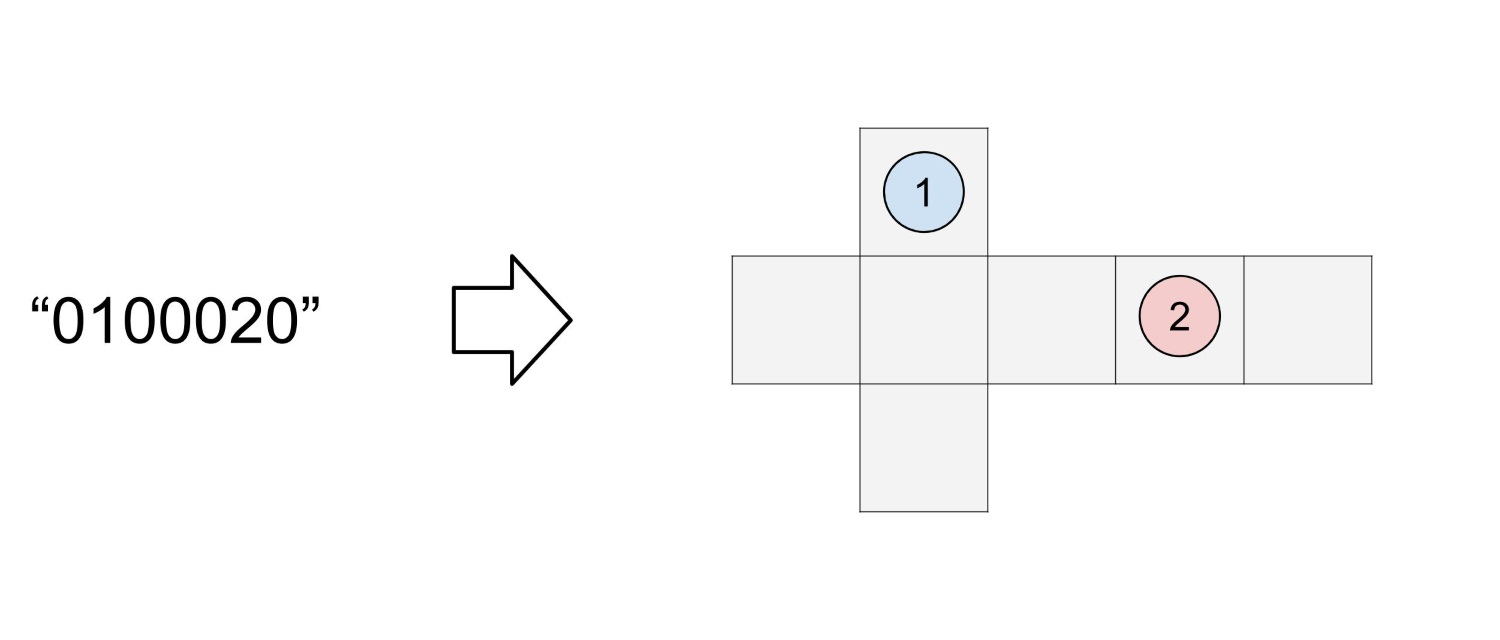
\includegraphics[height=4cm]{./Images/3_Playing_Field_Encoding.jpg}
        \caption{State string with equivalent playing field representation}
        \label{fig:field_mapping}
    \end{figure}


    The number of possible states is determined by the number of agents in the experiment and is equal to the number of unique permutations of agents and locations. It is calculated with the following formula:

    \begin{equation}
        N_{states} = \dfrac{m!}{(m-n)!}
    \end{equation}

    For an experiment with 1, 2 or 3 agents there are 7, 42 and 210 possible states, respectively. Given the somewhat low number of possible states, this study opted to implement the transition matrix as a direct state to state mapping, resulting in a square NxN matrix, N being the number of possible states. This trades a higher memory footprint for ease of implementation and interpretation. This particular implementation has a memory footprint proportional to N$^2$, in problems with a larger state space, one might opt to implement the transition table based on possible actions (Up, Right, Down, Left, and Stay) given that the matrix would increase to the order of N. Another, even more memory efficient implementation would be to store only the possible transitions in a list or dictionary. Given the sparse nature of the transition matrix, this option would greatly diminish the amount of memory necessary for running the learning process, at the expense of increased implementation complexity.

    Considering each agents only moves itself, the state transitions will be different for each agent. In this particular implementation it was decided to keep a separate transition table for each agent. These tables are calculated at the beginning of the experiment. For each agent, the program iterates over all the possible states and checks which moves are possible for said agent.

    The reward function grants agents 100 points for any action that transition them to the desired state, this includes the non-movement action of staying in the same place. Contrarily, agents are awarded negative 100 points for transitions that take them away from the desired state.

\section{Learning Policy} \label{sec:learning_policy}
    The learning policy selected for this study is the $\epsilon$-greedy policy. This policy relies on a dynamic value $\epsilon$, such that $0<\epsilon<1$, to determine an agent's strategy in a given state/time. The agent is to explore (i.e. take a random action) with $\epsilon$ probability, and exploit (i.e. take the action which has the highest expected return as per the Q-matrix) with (1-$\epsilon$) probability. The learning process starts with a predetermined $\epsilon$ value, which is gradually decreased after each learning episode. This means that when there is more uncertainty (i.e. at the beginning of the learning process, when not much is known regarding the environment), the agent is more prone to take random actions, exploring the possible state space and gathering feedback and "understanding" of the surrounding environment. Gradually, the more the agent knows regarding the environment, less often it takes random actions. This effectively has the result of directing the random exploration to regions surrounding the currently learned action policy. The selection of initial value and decay function for $\epsilon$ plays an important role in the performance of the learning process. If the decay is too slow, or the initial value is too high, the agent will keep exploring for longer possibly over exploring the problem space before converging to a policy, leading to longer training times. Conversely, if the decay is too fast (or the initial value is too low), the agent will converge to a policy faster, but this policy may be suboptimal as the problem space was underexplored. Naturally the optimal decay rate is dependent on the particular task being learned and the size of the state space. Striking this optimal balance is, therefore, an important step in the tuning process.

\section{Graphical Representation \& R Matrix} \label{sec:r_matrix}

    \begin{figure}[ht]
        \centering
        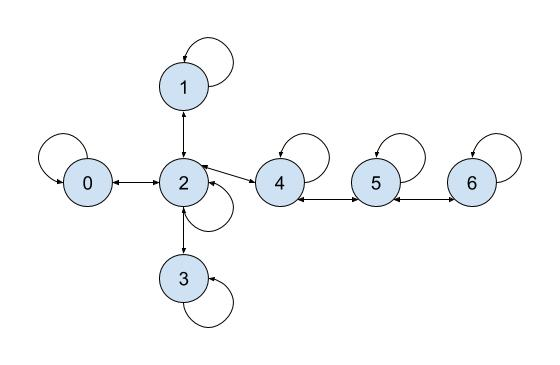
\includegraphics[height=4cm]{./Images/4_TransitionGraph.jpg}
        \caption{Base Transition Graph}
        \label{fig:transition_graph}
    \end{figure}

    The agents share the playing field and have the same movement rules, they also share a base movement graph. Figure \ref{fig:transition_graph} represent the shared transition graph between board locations. It is important to stress that, depending on the current board disposition, some transitions may not be available for a given agent. For example, an agent on location 6 may have it's 6$\rightarrow$5 transition blocked if there is another agent occupying location 5.

    As stated in section \ref{sec:transition}, the program makes use of this base transition graph to generate the full transition matrix. Since the study aims to analyze the behaviour of a multi-agent scenario, the agent's are deemed independent in terms of movement and policy. Hence, it was decided during implementation to have a separate transition matrix for each agent. Similarly, each agent has a separate R matrix associated with it. Even if, for the purposes of this study the agents are cooperative and share the same terminal state, their transitions into such final state are different given that their movement is ruled by the same constraints, but is not identical in terms of origin and destination states. The R matrixes are generated by the following steps:
    \begin{enumerate}
        \item Generate the transition matrix for that particular agent
        \item Set all transitions to have return of 0
        \item Set all transitions \textbf{away} from the desired terminal state to have reward of -100
        \item Set all transitions \textbf{into} the terminal state to 100
    \end{enumerate}

    Figure \ref{fig:r_matrix} shows the R matrix generated for agent \#1 in a experiment with a single agent.

    \begin{figure}[h]
        \centering
        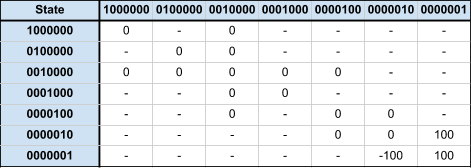
\includegraphics[height=4cm]{./Images/5_R_Matrix.png}
        \caption{R Matrix generated for experiment with a single agent}
        \label{fig:r_matrix}
    \end{figure}

\section{Q-Learning Parameters}
    The Q-Learning algorithm provides a some hyperparameters that may be tuned according to the task at hand and the limitations and opportunities associated with it. The two most prominent would be $\gamma$ and $\alpha$. This study presents additional parameters directly or indirectly related to Q-Learning (e.g. number of episodes, max steps per episode, $\epsilon$ decay rules), as well as parameters associated with the task itself (e.g. Number of agents, reward for reaching terminal state).

    \subsection{Discount Factor - $\gamma$}
        The discount factor ($\gamma$) main function is to weigh the probability of receiving expected future rewards. It is used as a multiplier to the maximum expected return of the next step, when updating the Q-Matrix. In a sense, it represents the certainty associated with eventually receiving future rewards. It's value may range from 0 to 1: 0 being no certainty at all, thus ignoring any expected return beyond the immediate step being taken. And 1 representing absolute certainty that future returns will match the expectation. For the initial experiment, $\gamma$ was set to \texttt{0.5}.

    \subsection{Learning Rate - $\alpha$}
        The learning rate parameter is used to control the rate at which the Q-Matrix is updated after a learning observation. As an analogy, it could be associated to the Q-Matrix's inertia. As with $\gamma$, $\alpha$'s values are between 0 and 1. As per the analogy, 0 would represent a scenario in which the Q-Matrix has infinite inertia, thus the Q-Matrix values remain the same, regardless of the feedback received from the observation. Oppositely, an $\alpha$ of 1 would represent a Q-Matrix with no inertia at all with it's values being completely replaced by the observations gathered at every step. For the initial experiment, $\alpha$ was set to \texttt{0.5}

    \subsection{Epsilon - $\epsilon$}
        The $\epsilon$ parameter refers to the $\epsilon$-greedy algorithm, which is used to select the actions taken by agents in the learning process. The results of such actions are then fed to the Q-Learning algorithm in the Q-Matrix update cycle. As stated in section \ref{sec:learning_policy} this experiment opted to rely on a commonly used pattern of multi-band $\epsilon$ decay. For the initial experiment the following values were used:
        \begin{itemize}
            \item Initial $\epsilon$: \texttt{0.999}
            \item Decay threshold (\texttt{r}): \texttt{0.5}
            \item Decay Rate 1 ($\epsilon$ $\geqslant$ \texttt{r}): \texttt{0.9995}
            \item Decay Rate 2 ($\epsilon$ $<$ \texttt{r} ): \texttt{0.995}
        \end{itemize}

    \subsection{Experiment duration - (\texttt{num\_episodes} and \texttt{max\_steps})}
        \sloppy This study defines two stopping criteria regarding the learning experiments: \texttt{num\_episodes} and \texttt{max\_steps}. The former determines how many learning episodes are ran in total before analyzing the results. While the latter establishes a maximum amount of steps taken in a single learning episode before declaring the agents as "stuck" and terminating the episode. If the terminal state is reached before \texttt{max\_steps} are taken, the episode is also terminated. One detail that is important to stress is that, in this experiment, in a multi-agent scenario the terminal state is only considered as reached when every single agent has performed an action that results in reaching that state, thus collecting its reward. For the initial experiment, the following values were used: \texttt{num\_episodes}=5000 and \texttt{max\_steps}=30.

    \subsection{Reward/Penalty}
        In this study, the reward and penalty values are defined arbitrarily, given the abstract nature of the experiment. As noted in section \ref{sec:r_matrix}, the initial values for reward and penalty are 100 and -100, respectively.

    \subsection{Number of Agents - (\texttt{num\_agents})}
        For implementation purposes, the number of agents in a experiment is also configurable. The initial experiments take place with both 1 and 2 agents settings.

\section{Q-Matrix Update Cycle}
    Central to the Q-Learning algorithm is the Q-Matrix update cycle. After each step taken by an agent, it's associated Q-Matrix is updated. The new value for the origin($s$)/action($a$) pair ($Q(s,a)_{new}$) is calculated based on the old origin/action value ($Q(s,a)_{old}$); the reward/penalty observed ($r$); the maximum expected return (as per the current Q-matrix) for future actions($a'$) taken from the destination state ($s'$) $\Rightarrow$ $max_{a'} Q(s',a')$; and the learning parameters discount factor ($\gamma$) and learning rate ($\alpha$). The equation used for updating the value is:

    \begin{equation}
        Q(s,a)_{new} = Q(s,a)_{old} + \alpha*[r+\gamma*max_{a'} Q(s',a') - Q(s,a)_{old}]
    \end{equation}

    Implementation-wise the code, in Python, used for updating the Q-Matrix is the following:

% Keep identation to left since \begin{python} respects current identation
    \begin{python}
def update_q_matrix(current_state, next_state, current_agent_id, earned_reward):
    # Get alpha and gamma from experiment settings
    alpha = EXPERIMENT['alpha']
    gamma = EXPERIMENT['gamma']

    # Get current agent's Q-matrix
    current_q = Q[current_agent_id]

    # Q(s,a)old
    old_expected_return = current_q.loc[current_state, next_state]

    # max a' Q(s',a')
    possible_next_moves = get_available_moves(next_state, current_agent_id)
    best_expected_return = max(current_q.loc[next_state, possible_next_moves])

    # Q(s,a)new
    new_expected_return = old_expected_return + alpha * (earned_reward + gamma * best_expected_return - old_expected_return)

    # Update value in current agent's Q-matrix
    current_q.loc[current_state, next_state] = new_expected_return
    \end{python}


\section{Initial Results}
\section{Further Tests}
\section{Quantitative Analysis}
\section{Qualitative Analysis}
\section{Error Correction Models}
\section{Error Correction Implementation Proposal}



\end{document}